\documentclass[../main]{subfiles}
\begin{document}
\setcounter{section}{4}
\section{画像}
%------------------------------------------------------------
\subsection{image*}
\Image[size=w0,caption={画像w0 (100\%)},label={fig:image_w0}]{H}{}{tuto-pbr-specular.png}
\Image[size=w8,caption={画像w8 (80\%)},label={fig:image_w8}]{H}{}{tuto-pbr-specular.png}
\Image[size=w6,caption={画像w6 (60\%)},label={fig:image_w6}]{H}{}{tuto-pbr-specular.png}
\Image[size=w4,caption={画像w4 (40\%)},label={fig:image_w4}]{H}{}{tuto-pbr-specular.png}
\Image[size=w2,caption={画像w2 (20\%)},label={fig:image_w2}]{H}{}{tuto-pbr-specular.png}
\begin{figure}[H]\begin{tikzpicture}
    \draw[fill,color=black!10!white] ({(.5-.05)*\textwidth}, .0\textheight) rectangle ({(.5+.05)*\textwidth}, .1\textheight);
    \draw (.0\textwidth, .0\textheight) -- (\textwidth, .0\textheight);
    \draw (.0\textwidth, .0\textheight) -- (.0\textwidth, .1\textheight) node[below right] {\small w0};
    \draw (\textwidth, .0\textheight) -- (\textwidth, .1\textheight) node[below left] {\small w0};
    \draw (.0\textwidth, .1\textheight) -- (\textwidth, .1\textheight);
    \foreach \i in {1,...,9}{
        \draw ({(.5-.05*\i)*\textwidth}, .0\textheight) -- ({(.5-.05*\i)*\textwidth}, .1\textheight) node[below right] {\small w\i};
        \draw ({(.5+.05*\i)*\textwidth}, .0\textheight) -- ({(.5+.05*\i)*\textwidth}, .1\textheight) node[below left] {\small w\i};
    }
\end{tikzpicture}\end{figure}
\begin{Code}{language=tex}
\Image[size=w0,caption={画像w0 (100\%)},label={fig:image_w0}]{H}{}{tuto-pbr-specular.png}
\Image[size=w8,caption={画像w8 (80\%)},label={fig:image_w8}]{H}{}{tuto-pbr-specular.png}
\Image[size=w6,caption={画像w6 (60\%)},label={fig:image_w6}]{H}{}{tuto-pbr-specular.png}
\Image[size=w4,caption={画像w4 (40\%)},label={fig:image_w4}]{H}{}{tuto-pbr-specular.png}
\Image[size=w2,caption={画像w2 (20\%)},label={fig:image_w2}]{H}{}{tuto-pbr-specular.png}
\end{Code}

\HRuleLeader
\subsection{frameimage*}
\Image[size=w4,frame,caption={画像w4 (40\%)},label={fig:frame_image_w4}]{H}{}{tuto-pbr-specular.png}
\Image[size=w2,frame,caption={画像w2 (20\%)},label={fig:frame_image_w2}]{H}{}{tuto-pbr-specular.png}
\begin{Code}{language=tex}
\Image[size=w4,frame,caption={画像w4 (40\%)},label={fig:frame_image_w4}]{H}{}{tuto-pbr-specular.png}
\Image[size=w2,frame,caption={画像w2 (20\%)},label={fig:frame_image_w2}]{H}{}{tuto-pbr-specular.png}
\end{Code}

%------------------------------------------------------------
\end{document}
